\begin{frame}{GATr - Introduzione}
    In diverse situazioni si ha a che fare con dati di natura geometrica, soprattutto
    in ambiti scientifici ed ingegneristici. Il vantaggio di utilizzare dati geometrici
    risiede nel comportamento definito dei dati sotto trasformazioni ben definite 
    (come distanze e rotazioni).

    Con l'obiettivo di utilizzare nel modo migliore questi dati, si introduce il 
    Geometric Algebra Transformer (GATr), un'architettura di rete general-purpose 
    che sfrutta dati geometrici. 
\end{frame}

\begin{frame}{GATr - Idee Chiave}
    GATr integra tre concetti fondamentali:
    \begin{itemize}
        \item \textbf{Algebra Geometrica}
        \item \textbf{Equivarianza}
        \item \textbf{Transformer}
    \end{itemize}
\end{frame}

\begin{frame}{Algebra Geometrica}

    Per rappresentare oggetti tridimensionali e applicare rotazioni e traslazioni su di 
    essi, la 3D GA non è sufficiente, poichè i multivettori dell'algebra tradizionale 
    possono rappresentare solo sottospazi lineari che passano per l'origine e rotazioni 
    intorno ad essa. 

    GATr consente di rappresentare i dati come multivettori dell'algebra geometrica 
    proiettiva \(\mathbb{G}_{3,0,1}\). In pratica lo spazio di interesse viene inserito 
    in uno spazio di dimensione superiore, aggiungendo una quarta coordinata omogenea 
    \(x_0 \Vb{e}_{0}\), ottenendo un'algebra di dimensione \(2^4 = 16\) dimensioni, capace di 
    rappresentare vari tipi geometrici e pose \(E(3)\).
\end{frame}

\begin{frame}{Algebra Geometrica}

    Nell’algebra geometrica, un vettore \( \Vb{u} \) può agire come operatore riflettendo 
    altri elementi nel piano ortogonale a \( \Vb{u} \). 
    Poiché ogni trasformazione ortogonale può essere espressa come una sequenza di riflessioni, 
    possiamo rappresentare qualsiasi trasformazione come prodotto geometrico di vettori 
    unitari, detti \textit{versori}  \( u = u_1 \cdots u_k \).

    Il prodotto di versori unitari genera un gruppo, chiamato \textit{Pin group}, 
    in cui i versori unitari si comportano come propri inversi (\( u^2 = 1 \)). 
    I prodotti di un numero pari di riflessioni formano il \textit{Spin group}. 
    Nell’algebra geometrica proiettiva \( \mathbb{G}_{3,0,1} \), questi gruppi 
    permettono di coprire le trasformazioni \( E(3) \) e \( SE(3) \), rispettivamente.
\end{frame}

\begin{frame}{Algebra Geometrica: Prodotto Sandwich}
    Le simmetrie tridimensionali (rotazioni, traslazioni, riflessioni) si rappresentano 
    con i multivettori di \( \mathbb{G}_{3,0,1} \). Il prodotto \textit{sandwich} applica 
    un versore \( u \) ad un elemento \( x \):

    \[
        \rho_u(x) = 
        \begin{cases}
            u x u^{-1} & \text{se } u \text{ è pari} \\
            u x \hat{u}^{-1} & \text{se } u \text{ è dispari}
        \end{cases}
    \]

    dove \( \hat{x} \) è l'involuzione di grado, che inverte il segno degli elementi 
    dispari (come vettori e trivettori) e lascia invariati quelli di grado pari. 
    Questo prodotto fornisce una rappresentazione lineare dei gruppi \textit{Pin} e 
    \textit{Spin}.

\end{frame}

\begin{frame}{Algebra Geometrica}

    Per rappresentare oggetti 3D, i piani sono descritti da vettori, e l'intersezione 
    di due oggetti geometrici è data dal prodotto wedge delle loro rappresentazioni. 
    Si crea una dualità tra oggetti e operatori, in cui gli oggetti 
    si comportano come trasformazioni che li lasciano invariati.

    La Tabella mostra una corrispondenza tra queste rappresentazioni, che risultano 
    compatibili con il prodotto \textit{sandwich} utilizzato per le trasformazioni.

\end{frame}

\begin{frame}{Algebra Geometrica: Tabella di Oggetti e Operatori}
    \begin{figure}
        \centering
        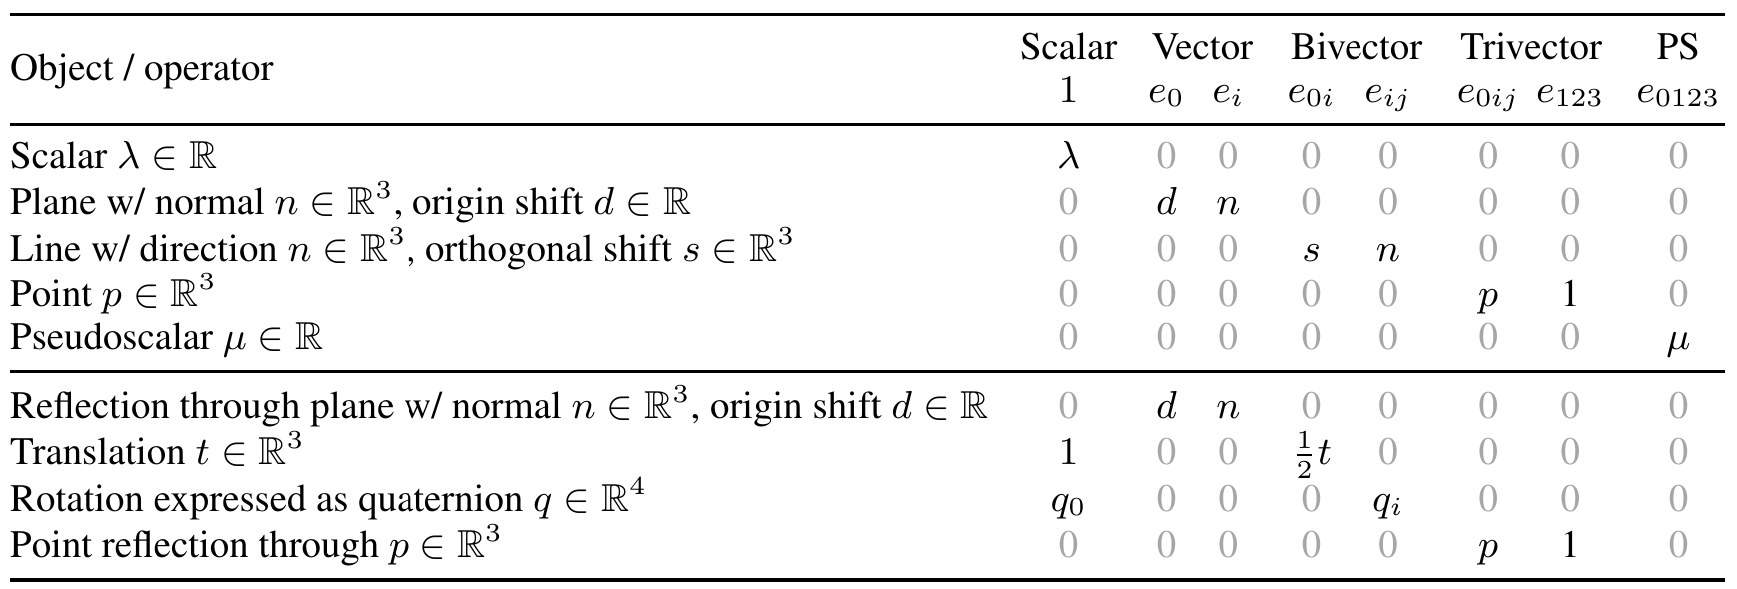
\includegraphics[width=0.9\textwidth]{../Images/relazioneOggettiOperatori.png}
        \caption{Tabella di oggetti 3D e trasformazioni}
        \label{fig:relazioneOggettiOperatori}
    \end{figure}
\end{frame}

\begin{frame}{Equivarianza}
    GATr è progettato per essere equivariante rispetto al gruppo di simmetria \(E(3)\), 
    che descrive le trasformazioni nello spazio tridimensionale. 

    A tale scopo, sono state sviluppate diverse nuove primitive 
    \(E(3)\)-equivarianti, tra cui mappe lineari equivarianti, un meccanismo di 
    attenzione, non-linearità e strati di normalizzazione.

    Vengono costruiti networks layers che sono equivarianti rispetto a \(E(3)\). 
    Una funzione \( f : \mathbb{G}_{3,0,1} \) è \( Pin(3,0,1) \)-equivariante rispetto
    alla rappresentazione \( p \) se 
    \[
        f(p_u(x)) = p_u(f(x))
    \]
    per ogni \( u \in Pin(3,0,1) \) e \(x \in \mathbb{G}_{3,0,1}\), dove \( p_u(x) \) è 
    il sandwich product definito in \eqref{eq:4}
\end{frame}

\begin{frame}{Trasformer}
    Per il GATr si è scelto di utilizzare l'architettura Transformer grazie alle sue 
    favorevoli proprietà di scalabilità, espressività, addestrabilità e versatilità.

    Di seguito si analizza più nel dettagli la struttura di questo modello.
\end{frame}

\begin{frame}{Principi di design}

    GATr è progettato per rappresentre vari oggetti e trasformazioni geometriche in 
    modo efficiente, permettendo il calcolo di diverse trasformazioni utilizzando pochi 
    strati e pochi dati. 

    GATr è stato progettato anche per essere simmetrico al gruppo di simmetria \(E(3)\),
    che include traslazioni, rotazioni e riflessioni. Permette quindi trasformazioni 
    arbitrarie sotto \(E(3)\), anche rispetto a traslazione degli input, permettendo di 
    rappresentare posizioni assolute. 

    GATr deve essere anche flessibile ripetto a più tipi di input geometrici, che vanno 
    da scene statiche a serie temporali. Il meccanismo di attenzione tramite prodotto 
    scalare, applicabile a più oggetti.

\end{frame}
\begin{frame}{Panoramica del Flusso di Lavoro di GATr}
    \begin{figure}
        \centering
        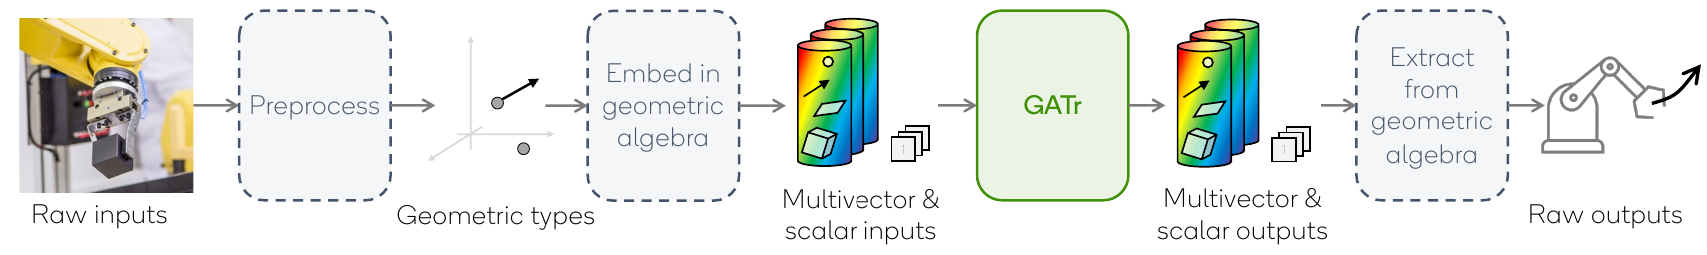
\includegraphics[width=1\textwidth]{../Images/GatrWorkflow.png}
    \end{figure}
    
    \textbf{Fasi del Flusso di Lavoro:}
    \begin{itemize}
        \item Se necessario gli input grezzi vengono preprocessati in tipi geometrici.
        \item Gli oggetti geometrici vengono incorporati in multivettori dell'algebra 
        geometrica \( G_{3,0,1} \), come descritto nella Figura \ref{fig:relazioneOggettiOperatori}.
        \item I dati multivettoriali vengono elaborati con una rete GATr.
    \end{itemize}
\end{frame}

\begin{frame}{Architettura di GATr}
    \begin{figure}
        \centering
        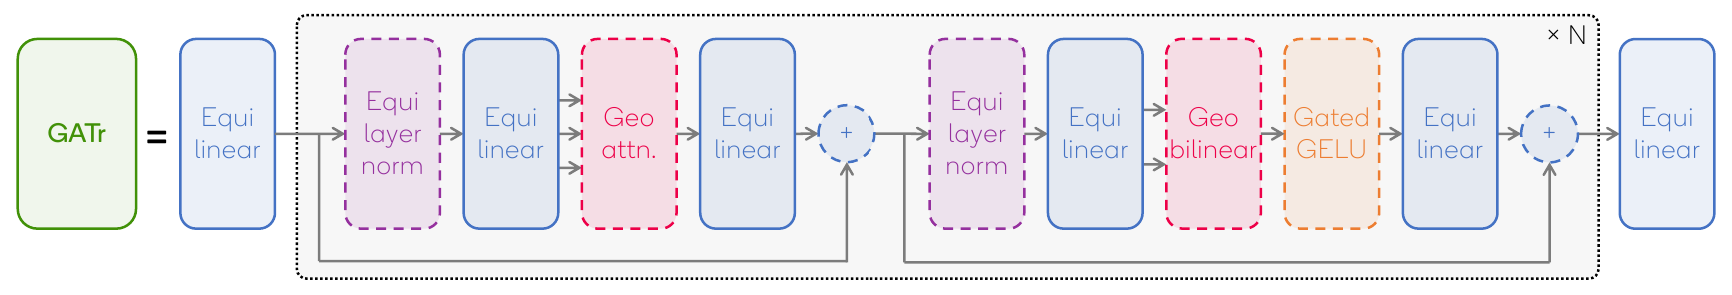
\includegraphics[width=1\textwidth]{../Images/GatrArchitecture.png}
        \caption{Architettura dettagliata di GATr.}
    \end{figure}
    
    L'architettura di GATr è composta da \( N \) blocchi trasformer, ognuno dei quali 
    include: un \textbf{LayerNorm} e un \textbf{meccanismo di auto-attenzione} per multivettori 
    equivarianti, una \textbf{connessione residua}, un altro LayerNorm, un \textbf{MLP con interazioni 
    bilineari geometriche} e una seconda connessione residua. 
    Dall’output di GATr si estraggono le variabili target, come illustrato in 
    Figura \ref{fig:relazioneOggettiOperatori}.
\end{frame}

\begin{frame}{LayerNorm - Layer Lineari}  
    Per preservare l’equivarianza, qualsiasi trasformazione lineare applicata ai 
    multivettori deve mantenere la coerenza sotto trasformazioni geometriche, come 
    rotazioni o traslazioni.

    \textbf{Formula Generale:}  
    \[
        \phi(x) = \sum_{k = 0}^{d+1} w_k {\langle x \rangle}_k + 
        \sum_{k = 0}^{d} v_k e_0 {\langle x \rangle}_k
    \]     

    \begin{itemize}
        \item La trasformazione combina diverse parti del multivettore, filtrate in base 
        al loro grado \( k \)
        \item \( w_k \) e \( v_k \) sono parametri apprendibili che controllano come 
        queste parti vengono combinate.
        \item \( e_0 \) funge da “base omogenea” per preservare la struttura geometrica.
    \end{itemize}
\end{frame}

% TODO: Approfondire e spiegare meglio 
\begin{frame}{Prodotti Geometrici Bilineari}
    (Da Approfondire).\\
    Per permettere alla rete di costruire nuove caratteristiche geometriche da quelle 
    esistenti, come il vettore di traslazione tra due punti, sono necessarie due 
    primitive aggiuntive. 
    \begin{itemize}
        \item \textbf{Prodotto geometrico} \(x, y \rightarrow xy \), consente di mescolare fa 
        loro diversi tipi di componenti geometriche, come vettori e piani.
        \item \textbf{Join} \( x,y \rightarrow (x^* \wedge y^*)^* \) operazione bilineare 
        che include il duale per rappresentare caratteristiche semplici come la distanza 
        euclidea. Il join viene reso equivariante anche rispetto alle riflessioni, 
        moltiplicandolo per uno pseudoscalare
    \end{itemize}
\end{frame}

\begin{frame}{Non-linearità e Normalizzazione}
    La non-linearità utilizzata è la Gated-GELU, applicata al componente scalare del 
    multivettore. La normalizzazione LayerNorm è \( E(3) \)-equivariante, calcolata su 
    canali con in prodotto interno invariati di \( \mathbb{G}_{3,0,1} \)
\end{frame}

\begin{frame}{Attenzione Multivettoriale Equivariante E(3)} 
    (Da Approfondire).\\
    L'attenzione multivettoriale equivariante E(3) è una versione adattata del meccanismo 
    di attenzione standard, progettata per lavorare con dati multivettoriali.

    Si parte da tensori di query, key e value, ciascuno con \( n_i \) elementi (o token) 
    e \( n_c \) canali.
    \begin{itemize}
        \item L'attenzione viene calcolata usando un prodotto interno scalato:
        \[
            \text{Attention}(q, k, v)_{i' c'} = \text{Softmax}_i 
            \left( \frac{\sum_i P_c \langle q_{i' c}, k_{i c} \rangle}{\sqrt{8 n_c}} \right) v_{i c'}
        \]
        \item Qui, \( \langle \cdot, \cdot \rangle \) è il prodotto interno invariante 
        dell’algebra geometrica \( G_{3,0,1} \), basato sul normale prodotto scalare \( R^8 \).
    \end{itemize}
    
\end{frame}

\begin{frame}{Estensioni dell'Architettura GATr}
    Diverse estensioni possono essere applicate all'architettura di GATr per aumentarne 
    la flessibilità e l'espressività:
    
    \begin{itemize}
        \item \textbf{Rappresentazioni scalari ausiliarie:}  
        Integrazione di dati non geometrici, come codifiche posizionali, con scalari 
        aggiuntivi.
        
        \item \textbf{Attenzione basata sulla distanza:}  
        Meccanismo di attenzione che considera la distanza euclidea tra i punti per 
        migliorare l'espressività del modello.
        
        \item \textbf{Incorporamenti posizionali:}  
        Utilizzo di embedding posizionali rotanti per sequenze di oggetti.
        
        \item \textbf{Attenzione assiale:}  
        Gestione di dati su più dimensioni (oggetti, sequenze temporali) attraverso 
        attenzione assiale.
    \end{itemize}
    
    Queste estensioni ampliano le capacità di GATr, mantenendo i benefici di 
    equivarianza ed efficienza computazionale.
\end{frame}



